\documentclass[fleqn]{article}
\usepackage{preamble}

\title{
	Differential Equations
}
\author{Abraham Murciano}

\begin{document}

\maketitle

\section{Section 1}

\begin{enumerate}[label=\textbf{\Alph*.}]
	\setlength{\itemsep}{\bigskipamount}
	\item
		Given a differential equation and a function \(y(x)\), we are to check that \(y\) is a solution to the differential equation.
		\begin{enumerate}
			\item[\textbf{1.}]
				For the following differential equation and function \(y(x)\),
				\[
					\dydx = 3y, \qquad y = 4e^{3x}
				\]

				Since we have \(y\), it can be differentiated to find \(\dydx\), then verify that it in fact is equal to \(3y\).
				\[
					\dydx = 12e^{3x} = 3 \cdot 4e^{3x} = 3y
				\]

			\item[\textbf{3.}]
				For the following differential equation and function \(y(x)\),
				\[
					\ddydxx + 16y = 0, \qquad y = \sin(4x)
				\]

				This time we must differentiate \(y\) twice to find \(\ddydxx\).
				\[
					\dydx = 4\cos(4x) \Rightarrow \ddydxx = -16\sin(4x)
				\]

				Now we can substitute this back into the original equation, and it quite obviously satisfies it.
				\[
					-16\sin(4x) + 16\sin(4x) = 0
				\]

			\item[\textbf{5.}]
				For the following differential equation and function \(y(x)\),
				\[
					\dydx + 2xy = 1, \qquad y = e^{-x^2} \int_0^x e^{t^2} dt + ce^{-x^2}
				\]
				we must find \(\dydx\).
				\begin{align*}
					\dydx & = e^{-x^2}e^{x^2} - 2xe^{-x^2} \int_0^x e^{t^2} dt - 2cxe^{-x^2} \\
					      & = e^0 - 2x \left(e^{-x^2} \int_0^x e^{t^2} dt + ce^{-x^2}\right) \\
					      & = 1 - 2xy
				\end{align*}

				Now we can substitute this into the original differential equation, and we see that is in fact satisfies it.
				\[
					\dydx + 2xy = 1 - 2xy + 2xy = 1
				\]

		\end{enumerate}

	\item
		\begin{enumerate}
			\item[\textbf{2.}]
				We are given the following differential equation.
				\[
					\dydx = 4xe^{2x}
				\]

				To find a solution, both sides can be integrated.
				\[
					y = 4 \int xe^{2x} dx
				\]

				Now integration by parts can be applied, with \(f(x) = x\) and \(g'(x) = e^{2x}\). This implies that \(f'(x) = 1\) and \(g(x) = \frac{1}{2}e^{2x}\). Therefore, by the rule of integration by parts,
				\[
					\int xe^{2x} dx = \frac{1}{2}xe^{2x} - \frac{1}{2} \int e^{2x} dx
				\]

				The next step is to calculate the integral of \(e^{2x}\). To do so, we will substitute \(u = 2x\).
				\[
					\int e^{2x} dx = \frac{1}{2} \int e^u du = \frac{1}{2} \cdot \frac{e^u}{\ln(e)} = \frac{1}{2} e^{2x} + c
				\]

				Therefore we have
				\begin{align*}
					y & = 4 \left(\frac{1}{2}xe^{2x} - \frac{1}{2} \left(\frac{1}{2} e^{2x}\right)\right) + c = 2xe^{2x} - e^{2x} + c \\
					  & = e^{2x} (2x-1) + c
				\end{align*}

				The graphs for \(y\) when \(c = 0\), \(1\), and \(-6\) can be seen in

				\begin{figure}[htb]
					\centering
					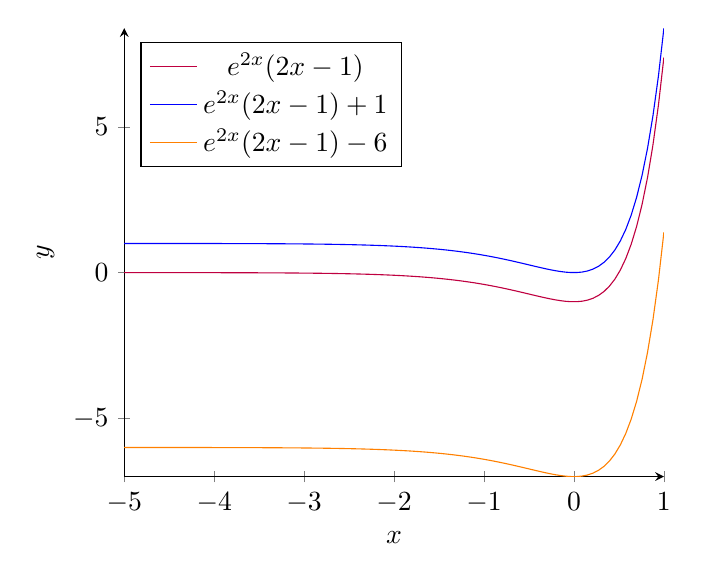
\begin{tikzpicture}
						\begin{axis}[
								legend pos=north west,
								axis lines = left,
								xlabel = \(x\),
								ylabel = \(y\),
							]
							\addplot [
								domain=-5:1,
								samples=100,
								color=purple,
							]
							{e^(2*x) * (2*x-1)};
							\addlegendentry{\(e^{2x} (2x-1)\)}
							\addplot [
								domain=-5:1,
								samples=100,
								color=blue,
							]
							{(e^(2*x) * (2*x-1)) + 1};
							\addlegendentry{\(e^{2x} (2x-1) + 1\)}

							\addplot [
								domain=-5:1,
								samples=100,
								color=orange,
							]
							{(e^(2*x) * (2*x-1)) - 6};
							\addlegendentry{\(e^{2x} (2x-1) - 6\)}

						\end{axis}
					\end{tikzpicture}
					\caption{\(y = e^{2x} (2x-1) + c\) when \(c = 0, 1,\) or \(-6\)}
					\label{qb2}
				\end{figure}


			\item[\textbf{4.}]
		\end{enumerate}
\end{enumerate}

\end{document}
